\chapter{Time Series Clustering}

\subsubsection*{What is a time series}
In this report we will deal with \textit{discrete time series}. 
A time series is defined as a set of observations $\{x_t\}$ recorded at a specific time $t$. 
A discrete time series is a time series where the set of times when observations are made ($T_0$) is discrete \cite{brockwell_davis_advanced}. 
A multivariate time series can be viewed as a set of vectors $\{\mathbf{x}_t\}$ where each set of vector elements $\{x^i_t\}$ is an individual time series. 
This means that the elements of the same vector $[x^1_t, x^2_t,...,x^N_t]$ are separate observations made at the same time instance $t$. 
In a wind turbine, measurements of the temperature in the gear box made every 10 seconds can be considered a univariate time series. 
While the set of measurements made every 10 seconds of the temperature in the gear box, the power produced by the turbine, and the wind speed ahead of the blades can be considered a multivariate time series. \bigskip

\section{Overview of Time Series Clustering}
There are three types of TSC, \textit{whole-series TSC}, \textit{subsequence TSC} and \textit{time-point TSC}. 
Whole-series TSC is when multiple ''whole'' time series are clustered with respect to each other. 
Subsequence TSC comprises the clustering of subsequences of the same time series with respect to each other. 
The defining difference between whole-series and subsequence TSC is that whole-series TSC clusters multiple time series while subsequence TSC clusters clusters different subsequences of the same time series. 
When performing time-point TSC the goal is to cluster individual observations of a time series wrt. to each other. 
In this review we will only consider work using whole-series TSC, so when the phrase \textit{time-series clustering} is used, one can assume that whole-series TSC is what is being refered to. \bigskip

TSC can be divided into three distinct parts: representation method, similarity metric and clustering algorithm. 
The choice of representation is key, and is the task of retaining the valuable information while disregarding the irrelevant information. As mentioned in section \ref{sec:objective}, only feature extraction based, and model based representation methods will be considered. 
The choice of similarity metric is important in a raw-data approach as it decides which aspects of the time series will be used to measure (dis)similarity, and has a has a significant impact on the time-complexity of the clustering system. 
However the requirements of similarity measure are somewhat relaxed in the feature-based and model-based approaches as the representation method already limits the number of aspects which one can compare time series with. 

%% SMALL SECTION ABOUT RAW-DATA BASED APPROACH, FEATURE BASED APPROACH AND MODEL BASED APPROACH.

\section{Time Series Models and Representations} \label{sec:ts_models}
To select suitable mathematical models for a dataset, we have to allow for the random nature of future observations. 
This is done by assuming that each observation in a time series $x_t$ is a realization of a particular random variable $X_t$. 
The time series can then be modelled as a collection/set of random variables $\{X_t\}$, also known as a \textit{stochastic process} \cite{brockwell_davis_advanced}. 
In the following subsections the theory of the three most prevalant feature extraction methods, and time series models will be presented: ARMA models, HMM and PCA.

\subsubsection*{Autoregressive Moving Average Models}
To define an ARMA model, one needs to have a clear understanding of the terms white noise process, and stationary process. 
We say that the stochastic process $\{Z_t\}$ is ''white noise'' with zero mean, and variance $\sigma^2$ ($\{Z_t\} \sim WN(0, \sigma^2)$) if and only if $\{Z_t\}$ is zero mean, and every random variable contained in $\{Z_t\}$ is uncorrelated with every other random variable contained in $\{Z_t\}$. 
A stochastic process $\{X_t\}$ is said to be weakly wide-sense stationary if the mean, and variance are constant for all terms in the process. 
$\{X_t\}$ is said to be weakly short-term stationary if the mean and variance of terms are constant for distinct time periods within the duration of the process, but are not constant for all terms in the process. 
For brevity the term ''stationary process'' will be used when refering to a \textit{weakly wide-sense stationary process}. 
An ARMA model descirbes a time series in terms of difference equations. 
It can be considered a combination of two smaller models, an autoregressive (AR) model and a moving average (MA) model. 
Let $\{X_t\}$ be a stationary process. 
An $\mathrm{MA}(q)$ model will describe every term $X_t$ as a linear combination of $q$ distinct white noise terms as in equation \eqref{eq:MA_q}.

\begin{equation}
    X_t = Z_{t} + \theta_1 Z_{t-1} + ... + \theta_q Z_{t-q}
    \label{eq:MA_q}
\end{equation}

Whereas an $\mathrm{AR}(p)$ model will describe every term $X_t$ as a linear combination of $p$ previous terms of $\{X_t\}$ as in equation \eqref{eq:AR_p}

\begin{equation}
    X_t = \phi_1 X_{t-1} + ... + \phi_p X_{t-p}
    \label{eq:AR_p}
\end{equation}

Putting equations \eqref{eq:AR_p} and \eqref{eq:MA_q} together, an $\mathrm{ARMA}(p,q)$ model will describe every term $X_t$ as a linear combination of $p$ previous terms, and $q$ white noise terms as in equation \eqref{eq:ARMA_p_q}.

\begin{equation}
    X_t - \phi_1 X_{t-1} - ... - \phi_p X_{t-p} = Z_{t} + \theta_1 Z_{t-1} + ... + \theta_q Z_{t-q}
    \label{eq:ARMA_p_q}
\end{equation}

Given that the polynomials $1 + \theta_1 z + \theta_2 z^2 + ... + \theta_q z^q$ and $1 - \phi_1 z - \phi_2 z^2 - ... - \phi_p z^p$ have no common factors \cite{brockwell_davis}.
When modelling a time series with an ARMA model, one usually attempts to decompose the time series into a set of components, as shown in equation \eqref{eq:ts_comp}. Here $X_t$ is the observed time series, $r_t$ is called the trend component, $s_t$ is called the seasonal component, $c_t$ is the cyclical component and $\epsilon_t$ is called the innovations component. 

\begin{equation}
    X_t = r_t + s_t + c_t + \epsilon_t
    \label{eq:ts_comp}
\end{equation}

$r_t$, $s_t$ and $c_t$ represent the deterministic components of trend, long term and short term periodic components of the time series respectively. $\epsilon_t$ represent the random component of the time series, and is often the component of the time series one attempts to model with an ARMA model. 

\subsubsection*{Hidden Markov Models} \label{s:hmm}
Let $\{X_n\}$ be a stochastic process where the random variables contained in $\{X_n\}$ only can take on a finite number of values which we will call states. 
Let $X_n$ denote the state at time period $n$. 
The probability of $X_n$ transitioning from state $i$ to state $j$ at the next time period $n+1$ is called the transition probability, and is denoted $p_{ij}$. 
It seems natural that $p_{ij}$ is conditional on what the state has been in previous time periods. 
$\{X_t\}$ is said to be a \textit{Markov chain} if $p_{ij}$ only is conditional on the past state, as shown in equation \eqref{eq:markov_property}.

\begin{equation}
    \begin{split}
        p_{ij}  &= P(X_n = i | X_{n-1} = i_{n-1}, X_{n-2} = i_{n-2},..., X_{1} = i_{1}, X_{0} = i_{0}) \\
                &= P(X_n = i | X_{n-1} = i_{n-1})      
    \end{split}
    \label{eq:markov_property}
\end{equation}

Suppose now that the states that the process is in are hidden from the observer. 
Instead there exists a finite set of signals $\{S\}$ that are emmitted when the process enters a state. 
For each state there is a set of \textit{emission probabilities} $P(S = s | X = j)$ associeted with a subset of the signals that can be emmitted.
In addition, let the probability of emmitting signal $s$, at time period $n$, in state $j$ ($P(S_n = s | X_n = j)$) be independent of previous states, and signals emmitted. 
A model of this type where the signals $S_1, S_2, ...$ are observed, and the underlying Markov states remain hidden is called a \textit{hidden Markov model} \cite{stoch_pros}. 

\subsubsection*{Principal Component Analysis and Independent Component Analysis}
There are two ways of reducing dimensionality in classification and regression tasks. 
One can choose to only use a subset of the dimensions given, or one can use a combination of the dimensions given.
PCA and ICA are both tools that reduce dimensionality by using a linear combination of the original dimensions given.
Consider a multivariate time series represented by the matrix $X$ with $n$ columns, where each column is a univariate time series of length $m$.
$X$ can then be reduced to a matrix of fewer columns of the same length by multiplying it with a projection matrix $W$, as in equation \ref{eq:reduce}. 
Let $Z$ represent the reduced matrix.
In PCA, the columns of $Z$ are called the \textit{principal components}, and in ICA they are called the \textit{independent components}. 

\begin{equation}
    Z = W X
    \label{eq:reduce}
\end{equation}

PCA and ICA is are methods for choosing $W$. 
In PCA $W$ is chosen in such a manner that the resulting dimensions are the dimensions with the highest variance.
The principal components are in fact the eigenvectors of the covarience matrix of $X$, so all the principal components are orthogonal. 
This is best illustrated graphically as in figure \ref{fig:pca_illustrated} where $w_1$ and $w_2$ illustrate the first and second principal components respectively.

\begin{figure}
    \begin{center}
    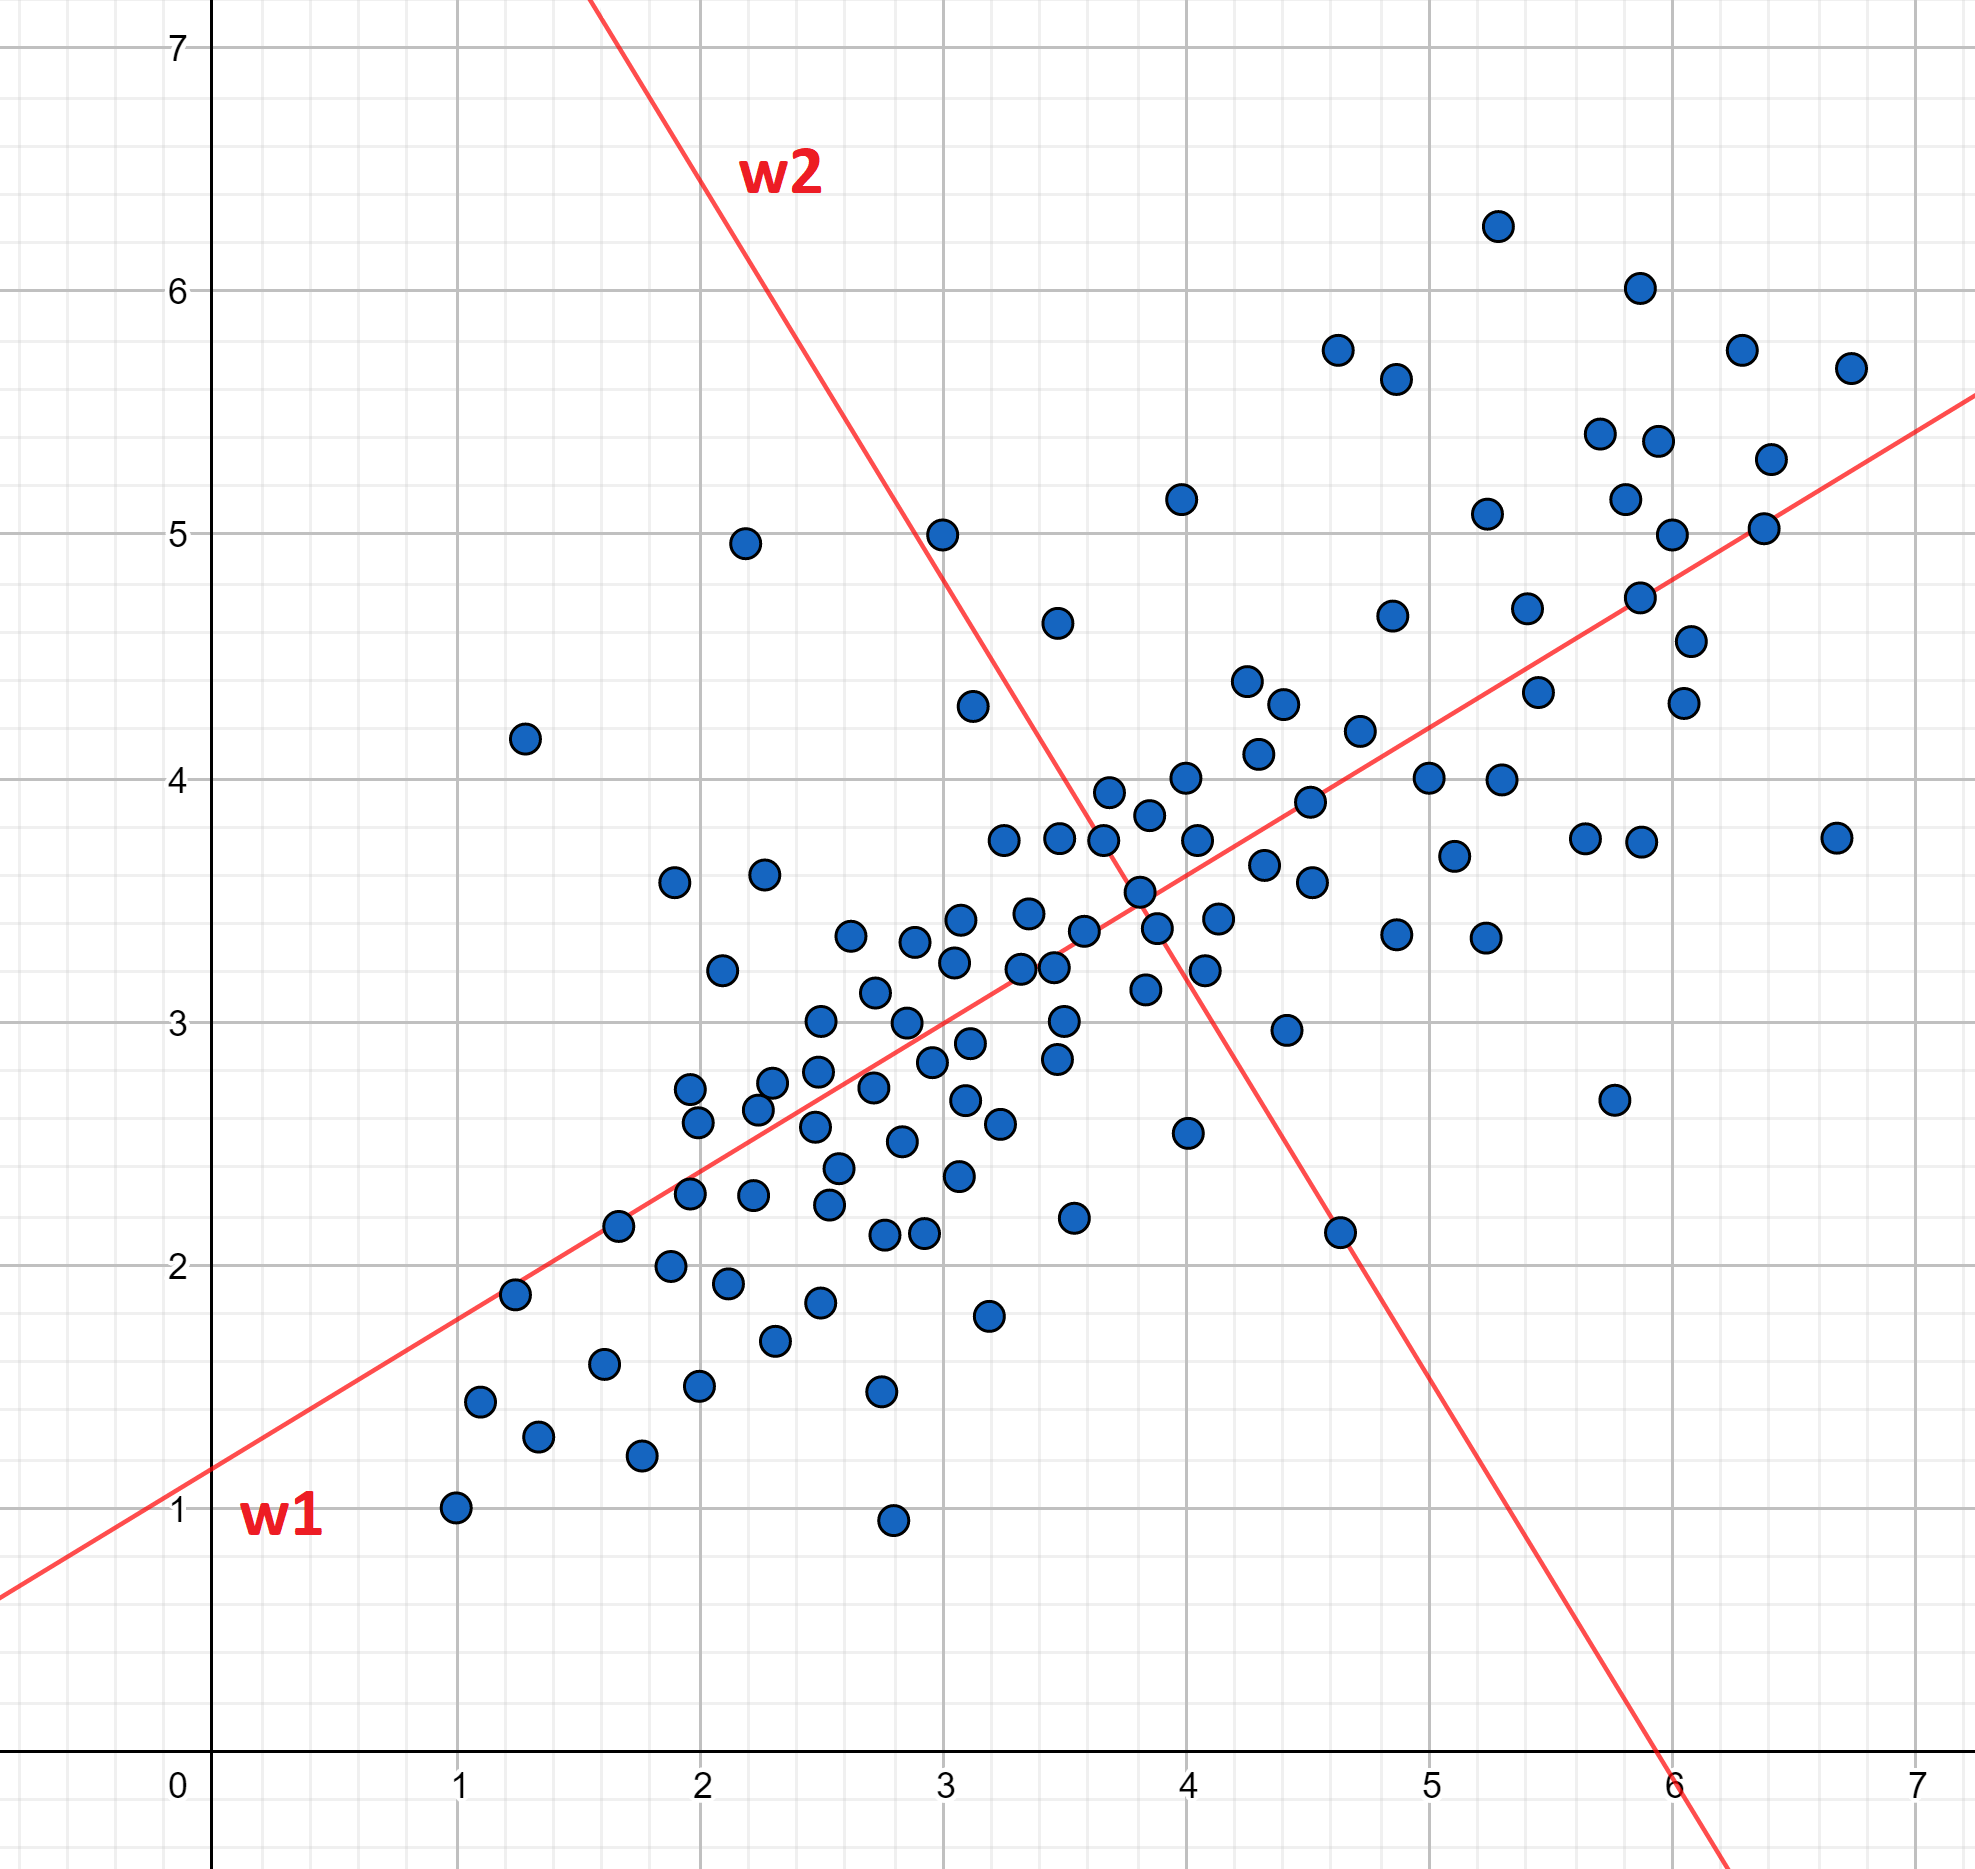
\includegraphics[width=0.4\textwidth]{tsc/pca_illustrated.png}
    \end{center}
    \caption{Illustration of how the principal components are found} 
    \label{fig:pca_illustrated}
\end{figure}

In ICA one assumes that the matrix of observed variables is a linear combination of mutually independent variables with an addition of noise, as illustrated in equation \ref{eq:ica_basics}. 
Where $X$ is the matrix of observed variables, $S$ is the matrix of independent hidden variables, $A$ is called a ''mixing matrix'' and $E$ is a noise matrix.  

\begin{equation}
    X = A S + E
    \label{eq:ica_basics}
\end{equation}

ICA is based upon the central limit theorem which states that a sum of random variables with arbitrary probability distributions will tend towards a Gaussian distribution. 
Hence, one chooses $W$ such that the resulting independent components are mutually independent and show as little Gaussian properties as possible.

\section{Representation Methods}
There are numerous ways which a time series can be represented. 
\textcite{tsc_rev} define a time series representation given time series data $\{x_t\} = \{x_1, x_2, ... ,x_T\}$ as transforming the time series into another vector $\{x_t\} = \{\hat{x}_1, \hat{x}_2, ... ,\hat{x}_L\}$ where $L < T$. 
In theory $L=T$, but most often the point in transforming a time series is to reduce the amount of information present in the raw time series to more easily reveal patterns of interest. \bigskip
% \input{tsc/rep_methods.tex}

\begin{table*}[h]
    \centering
    \ra{1.3}
    \begin{tabular}{p{0.45\textwidth}p{0.3\textwidth}}
        \toprule
        Feature extraction method & Articles \\
        \midrule
        PCA or ICA.                             & \cite{hysteresis_tsc_tensor_decomp, road_grade_china_pca_kmeans, load_tsc_state_space_model, multivariate_tsc_common_pca, ica_tsc_sea_level, copula_ica_tsc} \\
        % PCA                                   & \cite{hysteresis_tsc_tensor_decomp, road_grade_china_pca_kmeans, load_tsc_state_space_model, multivariate_tsc_common_pca} \\
        % ICA                                   & \cite{ica_tsc_sea_level, copula_ica_tsc} \\
        Time-frequency decomposition.           & \cite{shape_feat_mod_tsc_rfa, wavelet_multivar_tsc_multi_pca, ambient_air_vape_k_means, dwt_hac_kmeans_som, xml_dft_delaunay_traingulation, tsc_total_variation_distance, fragmented_periodogram, BSLEX_nonlin_nonstat_tsc}  \\
        % Wavelet transform.                    & \cite{shape_feat_mod_tsc_rfa, wavelet_multivar_tsc_multi_pca, ambient_air_vape_k_means, dwt_hac_kmeans_som, } \\
        % DFT.                                  & \cite{xml_dft_delaunay_traingulation, } \\
        % Spectral densities.                   & \cite{tsc_total_variation_distance} \\
        % Fragmented periodogram.               & \cite{fragmented_periodogram} \\
        % BSLEX.                                & \cite{BSLEX_nonlin_nonstat_tsc} \\
        Signal statistics.                      & \cite{ghsom_optimal_hedge_ratio, tsc_slaughterhouse, road_grade_china_pca_kmeans, auto_encoder_many_tsc_algorithms, } \\
        Matrix, or tensor decomposition.        & \cite{multivar_tsc_riemann_manifold, fuzzy_c_means_pso_svd, svd_birch_tsc_stock_price, hysteresis_tsc_tensor_decomp, tensor_multi_elastic_kernel_tsc} \\
        % Covarience matrices.                  & \cite{multivar_tsc_riemann_manifold, } \\
        % Singular value decomposition (SVD).   & \cite{fuzzy_c_means_pso_svd, svd_birch_tsc_stock_price, } \\
        % Tensor decomposition.                 & \cite{hysteresis_tsc_tensor_decomp, tensor_multi_elastic_kernel_tsc} \\
        Symbolic aggregate approximation (SAX). & \cite{clust_large_datasets_aghabozorg, apxdist_sax_k_modes, shape_feat_mod_tsc_rfa} \\
        Permutation based coding.               & \cite{dependency_tsc_energy_markets} \\
        Spline functions.                       & \cite{hier_clust_w_state_space_models} \\
        Topological feature extraction.         & \cite{topology_for_shape_based_tsc, } \\
        Autoencoder.                            & \cite{auto_encoder_many_tsc_algorithms} \\
        \bottomrule
    \end{tabular}
    \caption{Feature extraction based representation methods.}
    \label{tab:feat_repr_meth}
\end{table*}

Table \ref{tab:feat_repr_meth} summarizes the different feature extraction based representation methods encountered in literature. 
%% ICA and PCA
%% time frequency decomp
The category of time-frequency decomposition encompasses papers using the DWT, the continous wavelet transform, the DFT, spectral densities and fragmented periodograms.
\textcite{shape_feat_mod_tsc_rfa, ambient_air_vape_k_means, dwt_hac_kmeans_som} all use the DWT to decompose the time series signals. 
\textcite{shape_feat_mod_tsc_rfa} explores DWT as an alternative to other representation methods, while \textcite{ambient_air_vape_k_means, dwt_hac_kmeans_som} use DWT alone.
\textcite{fragmented_periodogram, BSLEX_nonlin_nonstat_tsc} both use periodograms to represent the time series to conserve some of the time-domain information about the signal. 
%% Matrix or tensor decomposition
The use of matrices or tensors to represent the time series was also found to be quite common. 
%% SAX and permutation based coding
In SAX, the time series is reduced by representing segments of specified length with symbols.
This is done to compress the length of the symbols. 
%% Permutation based
%% Spline functions 
%% Topological
%% Autoencoder
\textcite{auto_encoder_many_tsc_algorithms} compare a feature extraction based representation method, to a raw-data based approach. 
In the feature extraction based approach they train an autoencoder to reconstruct the time series used, then they separate the autoencoder into the encoder and the decoder parts. 
They then used the compressed features at the output of the encoder as the representation of the time series in the clustering tasks. 
They then go on to test a multitude of different clustering algorithms to cluster the compressed features. \bigskip

\begin{table*}[h]
    \centering
    \ra{1.3}
    \begin{tabular}{p{0.45\textwidth}p{0.3\textwidth}}
        \toprule
        Time series model & Articles \\
        \midrule
        ARMA model.                 & \cite{garch_robust_tsc, shape_feat_mod_tsc_rfa, temporal_tsc_threshold_ar_models, tsc_ar_metric_air_pollution, ar_metric_trimmed_fuzzy_tsc_pm10, moar_mpl_tsc, struct_damage_ar_fuzzy_c_means, fstar_hac_tsc, var_multivar_tsc} \\  
        HMM.                        & \cite{mixture_gaussian_hmm, hmm_pm10_quantifying_impacts, multivariate_tsc_hmm} \\
        State space model.          & \cite{stock_price_tsc_regr_trees_som, load_tsc_state_space_model} \\
        Varience ratio statistics.  & \cite{financial_tsc_variance_ratio, } \\
        Copula based model.         & \cite{copula_fuzzy_tsc_spatial} \\
        Network model.              & \cite{community_detection_networks_tsc, multivar_tsc_community_detection, } \\
        \bottomrule
    \end{tabular}
    \caption{Model based representation methods}
    \label{tab:model_repr_meth}
\end{table*}

%% ARMA Model
Table \ref{tab:model_repr_meth} shows the different model based representation methods encountered, 
as one can see the ARMA model is the representation method most frequently encountered. 
However, within this approach there is also great variety, especially with regard to model complexity.
\textcite{shape_feat_mod_tsc_rfa, struct_damage_ar_fuzzy_c_means, ar_metric_trimmed_fuzzy_tsc_pm10, tsc_ar_metric_air_pollution} fit the time series with an AR model, and use the similarity between the AR-coefficients to cluster the time series. 
\textcite{garch_robust_tsc} models the time series with a generalized AR conditional heteroscedasticity model, which is a variation of the ARMA model that is better suited for non-stationary time series. 
More specifically, in GARCH models one models the variance of the innovations component as an ARMA model itself. 
They then test different similarity metrics based on squared Euclidean distance between the model coefficients to cluster the time series. 
\textcite{temporal_tsc_threshold_ar_models, fstar_hac_tsc} both use forms of threshold AR models. 
Threshold AR models aim to describe non-linear time series by splitting the time series into operational regimes using a threshold variable, and then modeling the different regimes with different linear AR models \cite{temporal_tsc_threshold_ar_models}. \textcite{temporal_tsc_threshold_ar_models} then tests 22 different distance metrics to measure similarity between the model coefficients, which is then used to cluster the time series. \textcite{fstar_hac_tsc} on the other hand, use the Wald statistic to test whether to time series are from the same generative process, and use the p-value as a distance measure.
\textcite{moar_mpl_tsc} use AR models to represent different clusters, and cluster the different time series as to which AR model is the most likely generative process for a given time series, using the expectation-maximization algorithm.
%% HMM
\textcite{mixture_gaussian_hmm} have a very similar approach to \textcite{moar_mpl_tsc}, just that they use HMMs to represent the clusters, and cluster the time series with regard to which HMM is the most likely generative process. 
\textcite{hmm_pm10_quantifying_impacts} represent air pollution time series with a HMM. 
The states of the HMM correspond to different long-term states of pollution emission levels.
They cluster the different time series based on which ''polution emission state'' each time series is in at a particular time. 
\textcite{multivariate_tsc_hmm} model each time series with a HMM, and then calculate the Kullback-Liebler distance between the likelihood of different observation sequences given the state and specific HMM. 
%% State space
\textcite{load_tsc_state_space_model} represents user electricity-load time series with a state space model. Individual time series are treated as dynamical systems with states in phase space. 
The states are then represented with mapping functions, and uses the euclidean distance between parameters of the mapping functions to cluster time series. \textcite{stock_price_tsc_regr_trees_som} also explore the use of state space models, but to extract features of a time series.
%% Varience rato and Copula

%% Network model.

\newpage
\section{Similarity Metrics}
One similarity metric is Euclidean distance.
Another similarity metric is dynamic time warping.

\begin{table*}[h]
    \centering
    \ra{1.3}
    \begin{tabular}{p{0.45\textwidth}p{0.3\textwidth}}
        \toprule
        Similarity Metric & Articles \\
        \midrule
        Euclidean distance based metrics.   & \cite{financial_tsc_variance_ratio, hier_clust_w_state_space_models, topology_for_shape_based_tsc, community_detection_networks_tsc, shape_feat_mod_tsc_rfa, multivar_tsc_riemann_manifold, temporal_tsc_threshold_ar_models, ar_metric_trimmed_fuzzy_tsc_pm10, copula_ica_tsc, tsc_slaughterhouse, ambient_air_vape_k_means, dwt_hac_kmeans_som, xml_dft_delaunay_traingulation, svd_birch_tsc_stock_price, road_grade_china_pca_kmeans, fragmented_periodogram, auto_encoder_many_tsc_algorithms, load_tsc_state_space_model, struct_damage_ar_fuzzy_c_means, var_multivar_tsc, garch_robust_tsc, tsc_ar_metric_air_pollution, load_tsc_state_space_model,} \\
        % Squared Euclidean distance.       & \cite{garch_robust_tsc, } \\
        % Exponential Euclidean distance.   & \cite{tsc_ar_metric_air_pollution, load_tsc_state_space_model, } \\
        Other $p$-norms.                    & \cite{community_detection_networks_tsc, copula_fuzzy_tsc_spatial} \\
        Minkowski distance.                 & \cite{shape_feat_mod_tsc_rfa,} \\
        Tensor distance metric.             & \cite{hysteresis_tsc_tensor_decomp, } \\
        Matrix $L^p$ norms                  & \cite{tensor_multi_elastic_kernel_tsc} \\
        Dynamic time warping distance (DTW).& \cite{community_detection_networks_tsc, shape_feat_mod_tsc_rfa, temporal_tsc_threshold_ar_models} \\
        Approximate distance (APXDIST).     & \cite{clust_large_datasets_aghabozorg, apxdist_sax_k_modes} \\
        MINDIST.                            & \cite{shape_feat_mod_tsc_rfa, } \\
        Haussdorf distance.                 & \cite{temporal_tsc_threshold_ar_models, } \\
        Aggregated quasi-distance.          & \cite{BSLEX_nonlin_nonstat_tsc, } \\
        Kullback-Leibler distance.          & \cite{multivariate_tsc_hmm, } \\
        Total variation distance.           & \cite{tsc_total_variation_distance, } \\
        PCA similarity metric.              & \cite{wavelet_multivar_tsc_multi_pca} \\
        Information based metrics.          & \cite{dependency_tsc_energy_markets, } \\
        Pearson correlation coefficient.    & \cite{community_detection_networks_tsc, shape_feat_mod_tsc_rfa, fuzzy_c_means_pso_svd, } \\
        Test statistic.                    & \cite{fstar_hac_tsc} \\
        Principal component $R_e$.          & \cite{multivariate_tsc_common_pca} \\
        \bottomrule
    \end{tabular}
    \caption{}
    \label{tab:}
\end{table*}

\section{Clustering Algorithms}
As mentioned before clustering is a form of unsupervised machine learning. 
The goal is to divide the dataset into clusters, by maximizing some similarity metric for members of the same cluster, and minimizing the same metric for members of different clusters.

\begin{table*}[h]
    \centering
    \ra{1.3}
    \begin{tabular}{p{0.45\textwidth}p{0.3\textwidth}}
        \toprule
        Clustering Algorithm & Articles \\
        \midrule
        Expectation maximization 			& \cite{mixture_gaussian_hmm, moar_mpl_tsc, auto_encoder_many_tsc_algorithms} \\
        Hierarchical clustering 			& \cite{financial_tsc_variance_ratio, hier_clust_w_state_space_models, BSLEX_nonlin_nonstat_tsc, shape_feat_mod_tsc_rfa, ica_tsc_sea_level, multivar_tsc_riemann_manifold, tsc_total_variation_distance, dependency_tsc_energy_markets, copula_ica_tsc, tsc_slaughterhouse, dwt_hac_kmeans_som, auto_encoder_many_tsc_algorithms, fstar_hac_tsc, } \\
        K-means family 						& \cite{financial_tsc_variance_ratio, hier_clust_w_state_space_models, topology_for_shape_based_tsc, multivariate_tsc_hmm, apxdist_sax_k_modes, temporal_tsc_threshold_ar_models, ambient_air_vape_k_means, hysteresis_tsc_tensor_decomp, dwt_hac_kmeans_som, road_grade_china_pca_kmeans, auto_encoder_many_tsc_algorithms} \\
        Fuzzy C-means family 				& \cite{garch_robust_tsc, copula_fuzzy_tsc_spatial, temporal_tsc_threshold_ar_models, tsc_ar_metric_air_pollution, wavelet_multivar_tsc_multi_pca, ar_metric_trimmed_fuzzy_tsc_pm10, fuzzy_c_means_pso_svd, struct_damage_ar_fuzzy_c_means, } \\
        Self-organizing map (SOM) 			& \cite{ghsom_optimal_hedge_ratio, stock_price_tsc_regr_trees_som, dwt_hac_kmeans_som, } \\
        % HMM                                   & \cite{hmm_pm10_quantifying_impacts} \\ % hvis du først skal ha med state space kan du også ha med HMM
        % State space model 					& \cite{hier_clust_w_state_space_models} \\
        % Community detection algorithms		& \cite{community_detection_networks_tsc} \\
        Custom algorithms 					& \cite{clust_large_datasets_aghabozorg, multivariate_tsc_common_pca, tensor_multi_elastic_kernel_tsc, var_multivar_tsc} \\
        Spectral clustering 				& \cite{temporal_tsc_threshold_ar_models, fragmented_periodogram, auto_encoder_many_tsc_algorithms, } \\
        % Matrix factorization 				& \cite{multivar_tsc_community_detection} \\
        Delauney Triangulation method 		& \cite{xml_dft_delaunay_traingulation} \\
        BIRCH 								& \cite{svd_birch_tsc_stock_price, auto_encoder_many_tsc_algorithms, } \\
        Affinity propagation  				& \cite{auto_encoder_many_tsc_algorithms} \\
        DBSCAN  							& \cite{auto_encoder_many_tsc_algorithms} \\
        Mean shift  						& \cite{auto_encoder_many_tsc_algorithms} \\
        \bottomrule
    \end{tabular}
    \caption{Clustering algorithms}
    \label{tab:clust_alg}
\end{table*}

\section{Discussion}
